\subsubsection{Effect of Pileup on Dijet Balance}

The \pt{} balance of dijets events can be used to construct a correction factor or used to ascertain aspects of the JES uncertainty \cite{ref:JES}.
In this section it is used as a cross-check of JES uncertainty components from pileup.
This is done by calculating the relative response for events with different levels of pileup.

Two estimators of the amount of pileup used are the number of primary vertices, NPV, and the mean number of interactions per bunch crossing, $\mu$.
Figure \ref{JetPerf:NPV_Mu} shows (a) the NPV distribution and (b) the $\mu$ distributions.
These NPV and $\mu$ cuts are chosen to select events with different amount of pileup.
For the NPV cuts, three slices are chosen so that each has good statistics, but also has differences in the average NPV per slice.
Three NPV regions are defined to select different pileup conditions, \Range{NPV}{0}{2}, \Range{NPV}{3}{6}, and  $\rm NPV\ge7$, with an average NPV of 2.48, 4.48 and 7.71 respectively. 
For the $\mu$ cuts, two slices are chosen, one that includes the peak, and one that includes the tail, both with good statistics. 
Two $\mu$ regions are defined, \Range{\mu}{0}{7} and  $\mu > 7$, with an average $\mu$ of 5.33 and 9.94 respectively. 
Data points which have no cuts on $\mu$ or NPV are also shown for comparative purposes.
These have an average NPV and $\mu$ of 5.19 and 6.48 respectively.



%High NPV:  Ave NVP:  7.71314
%Med NPV:  Ave NVP:  4.48111
%Low NPV:  Ave NVP:  2.47613
%Standard: Average mu : 6.47532  Ave NVP:  5.18579


Figures \ref{JetPerf:PileupComp_j10}, \ref{JetPerf:PileupComp_j15} and \ref{JetPerf:PileupComp_j20}  show the relative response as a function of detector $\eta$ for jets with $22<\ptave{}<30$ GeV, $30<\ptave{}<40$ GeV and $55<\ptave{}<75$ GeV, respectively, for different NPV ranges.
For the $22<\ptave{}<30$ GeV jets, the relative response in the forward bins is lower for jets in the low pileup conditions than the jets using the full data.
The medium has a higher relative response in the bins oustide the reference region.
The spread of the three different NPV points is contained within $\sim 4\%$ and there is no systematic difference in spread as a function of $\eta{}$.
For the $30<\ptave{}<40$ GeV jets, the spread has decreased to within $\sim 2\%$. 
In the forward bins at negative $\eta$, the low pileup and high pileup have a higher and lower response than the average respectively, however this is probably just fluctuations as there is no patheological effect.
For the  $55<\ptave{}<75$ GeV jets, the spread is within $\sim 1\%$, and there is no obvious trend in the differences between the different pileup conditions.

The observation that the low \ptave{} jets are affected more, is not unexpected, as pileup can be considered to add a fixed amount of additional energy per additional proton-proton interaction.
This additional energy will be a larger fraction of a low \pt{} jet than a high \pt{} jet at the same rapidity, and so the net effect will be larger.
Naively, it might be expected that the jets in the lower pileup conditions should have a lower relative response than jets in a higher pileup condition, however the EM+JES calibration does an pileup offset correction, which should account for this.


Figures \ref{JetPerf:MuComp_j10}, \ref{JetPerf:MuComp_j15} and \ref{JetPerf:MuComp_j20}  show the relative response as a function of detector $\eta$ for jets with $22<\ptave{}<30$ GeV, $30<\ptave{}<40$ GeV and $55<\ptave{}<75$ GeV respectively for different $\mu$ ranges.
For the $22<\ptave{}<30$ GeV jets, the spread  is $\sim 3\%$ for $-2.8\le\eta\le-2$ range, but for most bins it is within $ 1-2\%$.
In most of the bins the low pileup sample has a responses slightly higher than the response from the high pileup samples.
For the $30<\ptave{}<40$ GeV jets, the relative responses are closer to unity than for the lower \ptave{} jets.
The spread is consistent $2\%$ with approximately equal number of bins where the low pileup sample is above the high pileup sample, than the reverse.
For the $55<\ptave{}<75$ jets, the spread is $<1\%$ for all but one bin, and the relative response is close to one.  
As with the assessment of the pileup using the NPV, the spread shows a general downwards trend for higher \ptave{}, though the jets with $30<\ptave{}<40$ GeV have a marginally higher spread than $22<\ptave{}<30$ GeV, but without the larger fluctuations,

The observed effects from NPV and $\mu$ are $~3-4\%$ for low \ptave{} jets, and reduce to $~1\%$ for jets with $55<\ptave{}<75$.
These spreads of values for the relative response show agreement to the JES uncertainty due to pileup using the method described in \cite{ref:Pileup} and combined to the JES uncertainty in \cite{ref:JES2011}.



\begin{figure}
\centering
\mbox{
              \subfigure[]{\epsfig{figure=figures/JetPerformance/2011/NPVDist.eps,width=0.5\textwidth}}\quad
              \subfigure[]{\epsfig{figure=figures/JetPerformance/2011/MuDist.eps,width=0.5\textwidth}}\quad
                              }
\caption[Number of primary vertices and $\mu{}$ for 2011 data]{
(a) The NPV distribution and (b) the $\mu$ distribution for 2011 data.
\label{JetPerf:NPV_Mu}}
\end{figure}



\begin{figure}
\centering
\mbox{
              \epsfig{figure=figures/JetPerformance/2011/ResponseNPVj10Comp.eps,width=0.9\textwidth}
}
\caption[Relative response as a function of $\eta$ for 3 different pileup conditions, based on NPV, for jets with $22<\ptave{}<30$ GeV]{
Relative response as a function of detector $\eta$ for jets with $22<\ptave{}<30$ GeV.
Relative responses are shown for events with \Range{NPV}{0}{2}, \Range{NPV}{3}{6}, $\rm NPV\ge7$ and all NPV. 
\label{JetPerf:PileupComp_j10}}
\end{figure}



\begin{figure}
\centering
\mbox{
              \epsfig{figure=figures/JetPerformance/2011/ResponseNPVj15Comp.eps,width=0.9\textwidth}
              %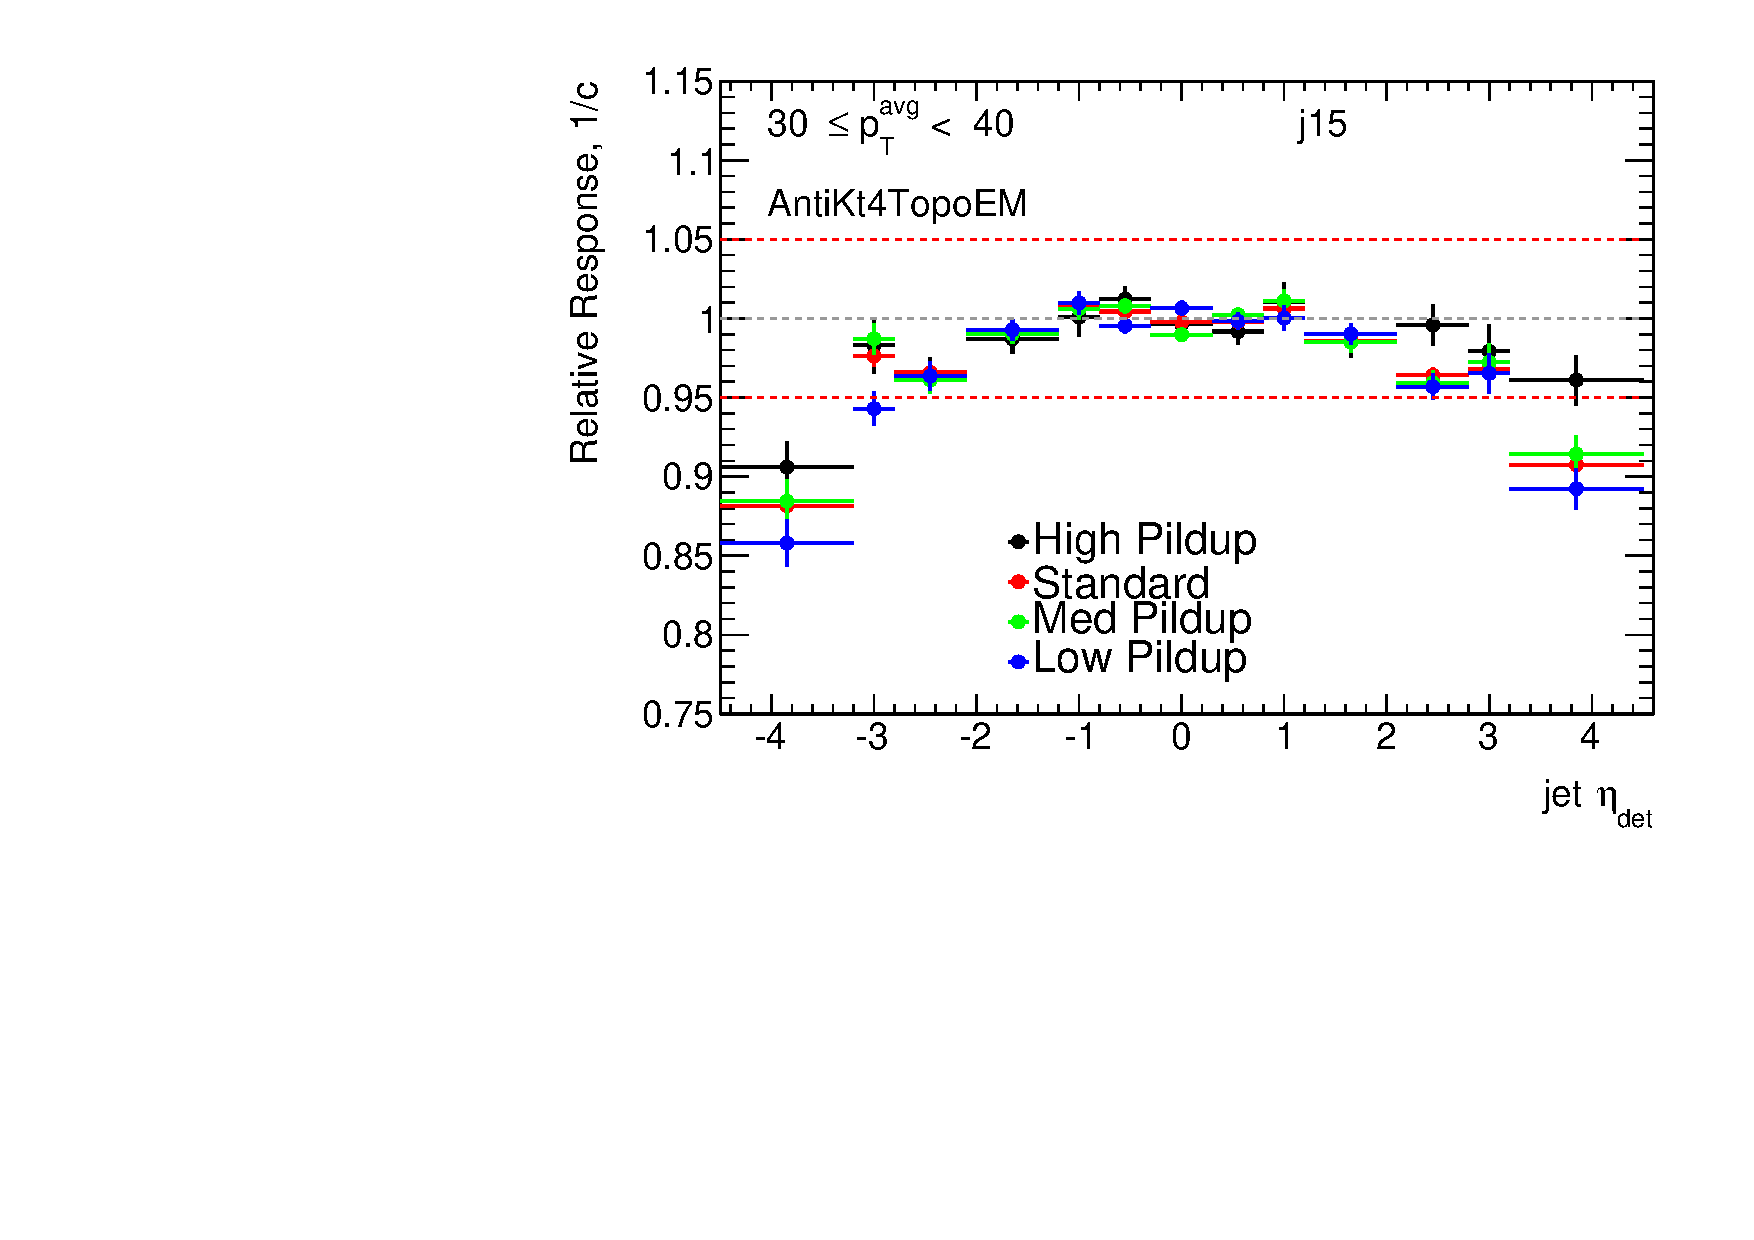
\includegraphics[width=0.8\textwidth]{figures/JetPerformance/2011/Pileup/PileupComp_AntiKt4TopoEM_j15_30-40Uncorrected.pdf}
}
\caption[Relative response as a function of $\eta$ for 3 different pileup conditions, based on NPV, for jets with $30<\ptave{}<40$ GeV]{
Relative response as a function of detector $\eta$ for jets with $30<\ptave{}<40$ GeV.
Relative responses are shown for events with \Range{NPV}{0}{2}, \Range{NPV}{3}{6}, $\rm NPV\ge7$ and all NPV. 
\label{JetPerf:PileupComp_j15}}
\end{figure}

\begin{figure}
\centering
\mbox{
              \epsfig{figure=figures/JetPerformance/2011/ResponseNPVj30Comp.eps,width=0.9\textwidth}
              %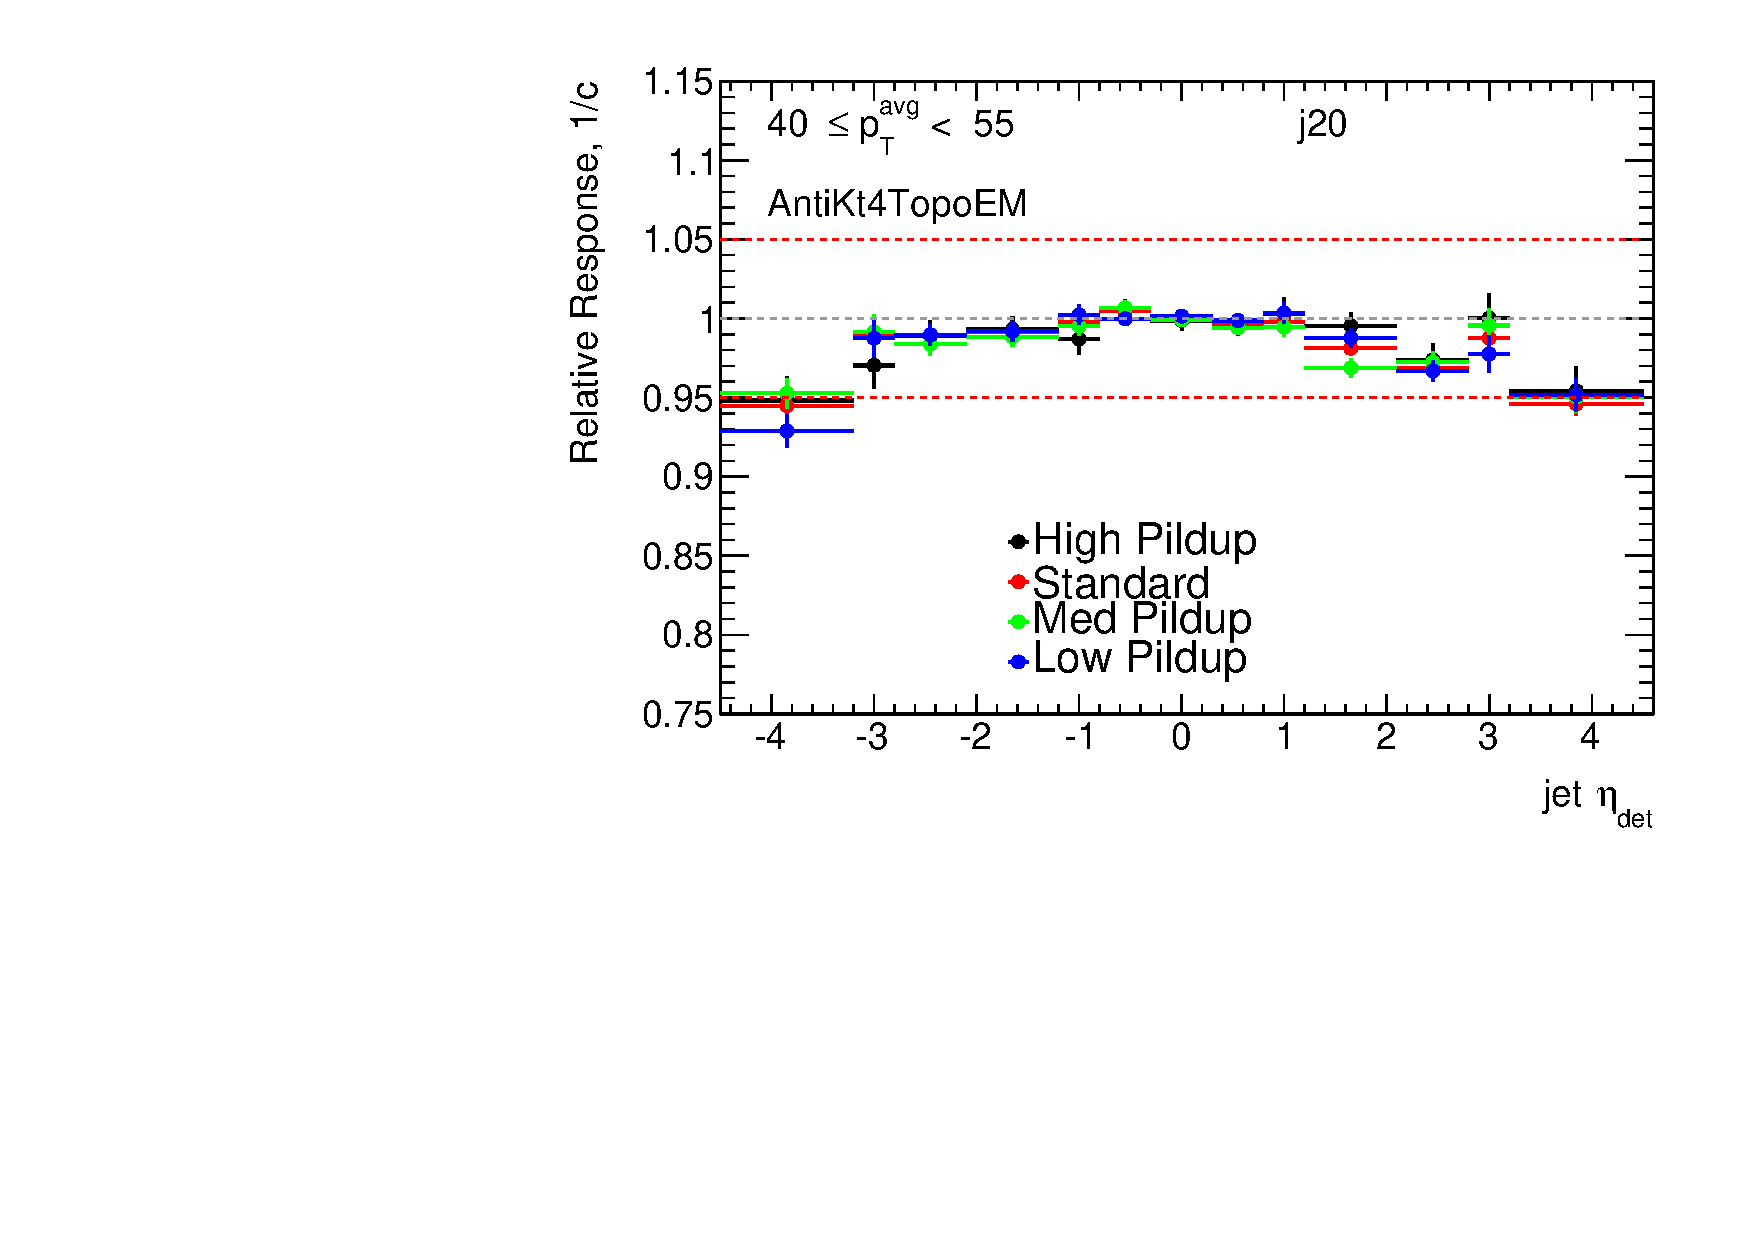
\includegraphics[width=0.8\textwidth]{figures/JetPerformance/2011/Pileup/PileupComp_AntiKt4TopoEM_j20_40-55Uncorrected.pdf}
}
\caption[Relative response as a function of $\eta$ for 3 different pileup conditions, based on NPV, for jets with $55<\ptave{}<75$ GeV]{
Relative response as a function of detector $\eta$ for jets with $55<\ptave{}<75$ GeV.
Relative responses are shown for events with \Range{NPV}{0}{2}, \Range{NPV}{3}{6}, $\rm NPV\ge7$ and all NPV. 
\label{JetPerf:PileupComp_j20}}
\end{figure}

\begin{figure}
\centering
\mbox{
              \epsfig{figure=figures/JetPerformance/2011/Responsemuj10Comp.eps,width=0.9\textwidth}
              %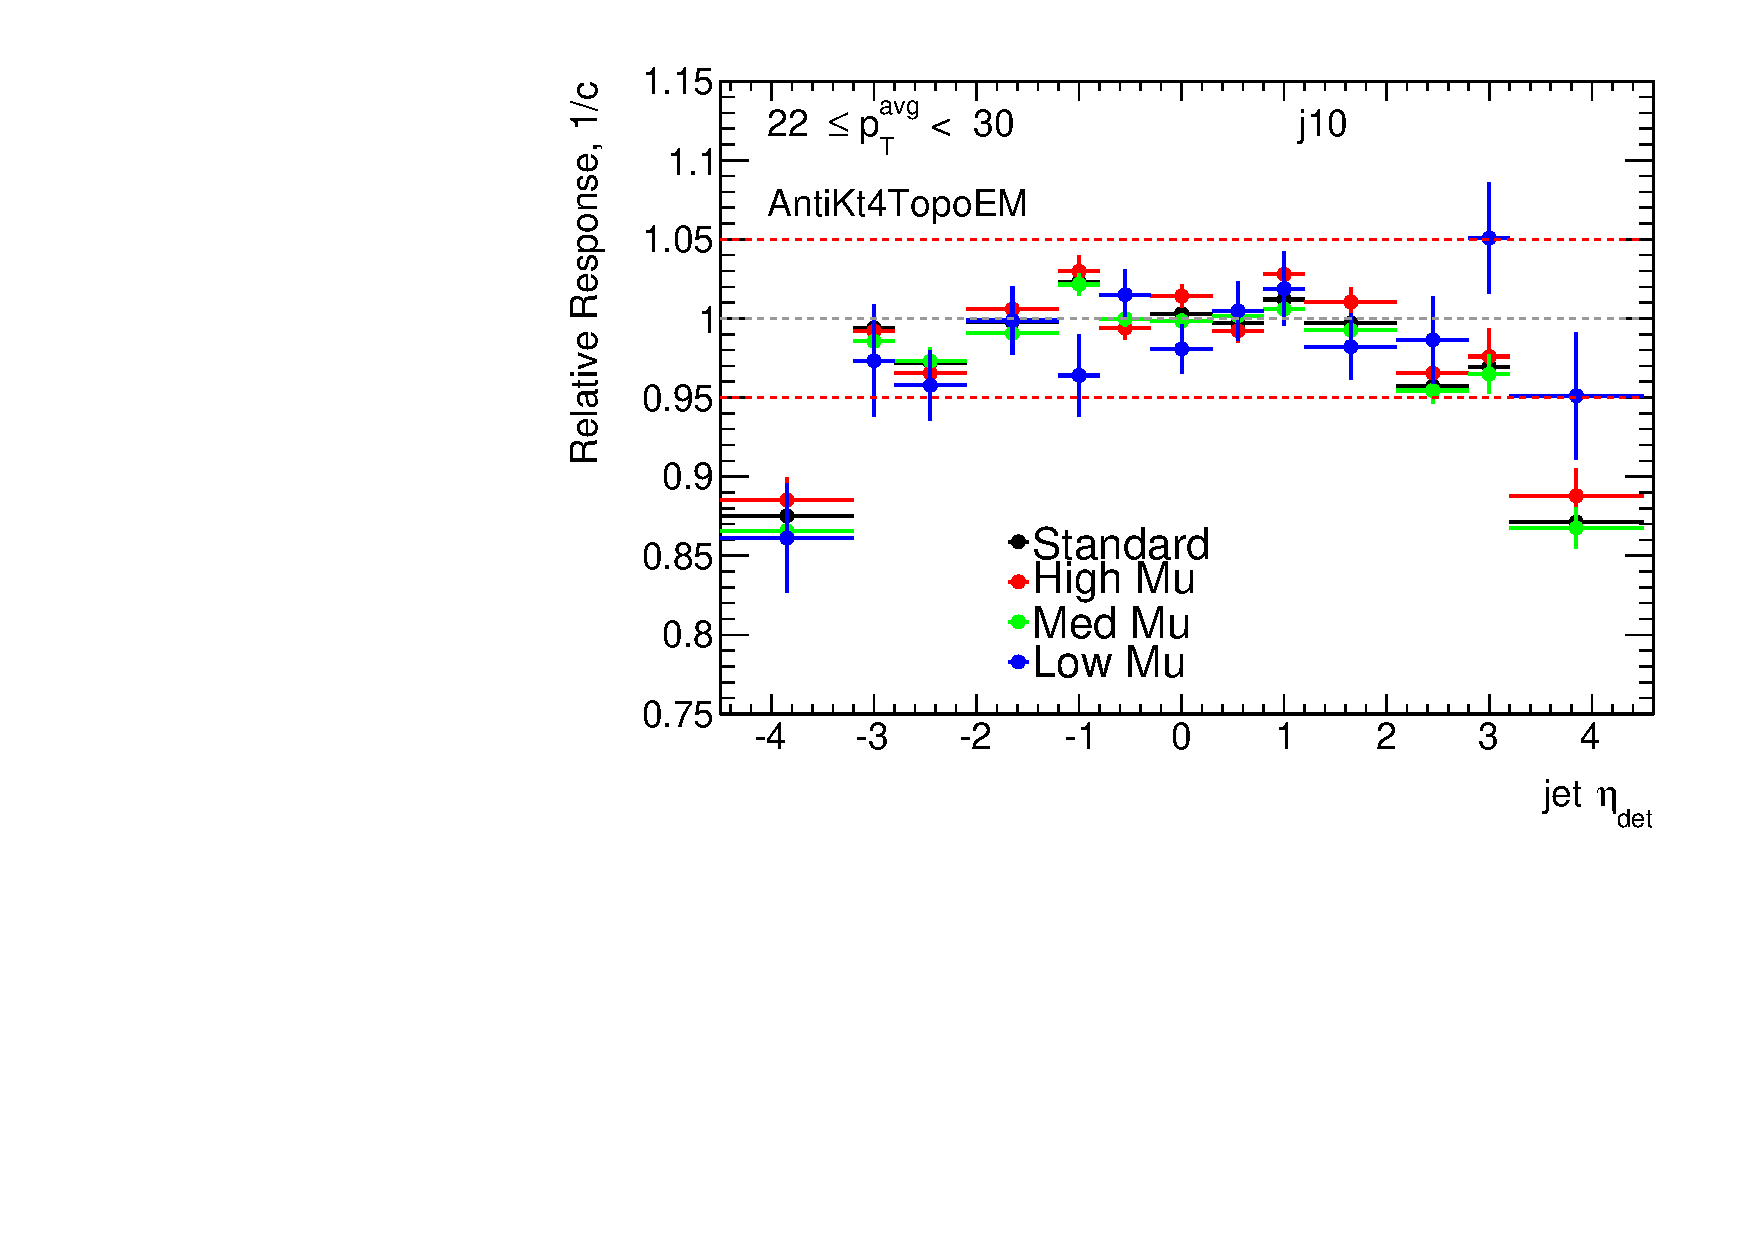
\includegraphics[width=0.8\textwidth]{figures/JetPerformance/2011/Pileup/MuComp_AntiKt4TopoEM_j10_22-30Uncorrected.pdf}
}
\caption[Relative response as a function of $\eta$ for 2 different pileup conditions, based on $\mu{}$, for jets with $22<\ptave{}<30$ GeV]{
Relative response as a function of detector $\eta$ for jets with $22<\ptave{}<30$ GeV.
Relative responses are shown for events with \Range{\mu}{0}{6}, $\rm \mu\ge6$ and all $\mu$. 
\label{JetPerf:MuComp_j10}}
\end{figure}



\begin{figure}
\centering
\mbox{
              \epsfig{figure=figures/JetPerformance/2011/Responsemuj15Comp.eps,width=0.9\textwidth}
              %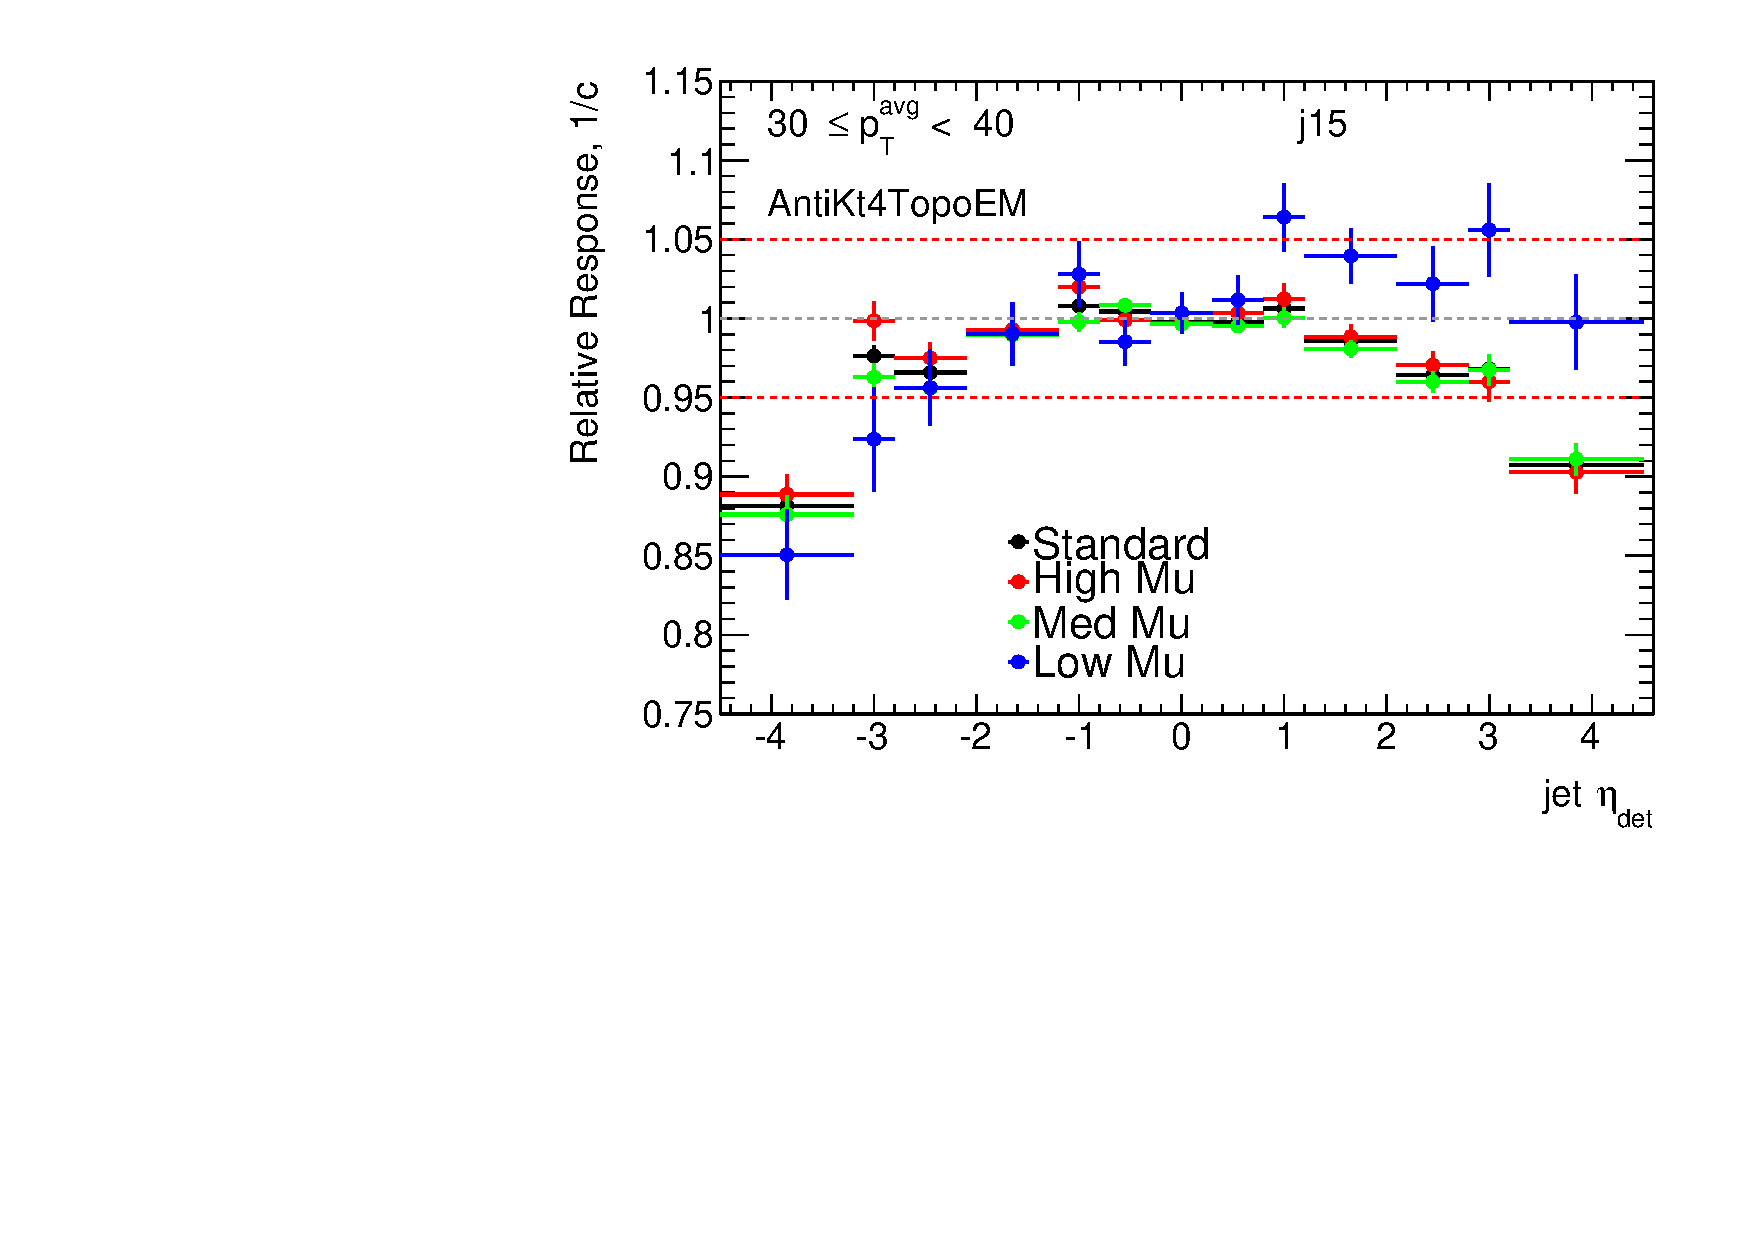
\includegraphics[width=0.8\textwidth]{figures/JetPerformance/2011/Pileup/MuComp_AntiKt4TopoEM_j15_30-40Uncorrected.pdf}
}
\caption[Relative response as a function of $\eta$ for 2 different pileup conditions, based on $\mu{}$, for jets with $30<\ptave{}<40$ GeV]{
Relative response as a function of detector $\eta$ for jets with $30<\ptave{}<40$ GeV.
Relative responses are shown for events with \Range{\mu}{0}{6}, $\rm \mu\ge6$ and all $\mu$. 
\label{JetPerf:MuComp_j15}}
\end{figure}

\begin{figure}
\centering
\mbox{
              \epsfig{figure=figures/JetPerformance/2011/Responsemuj30Comp.eps,width=0.9\textwidth}
              %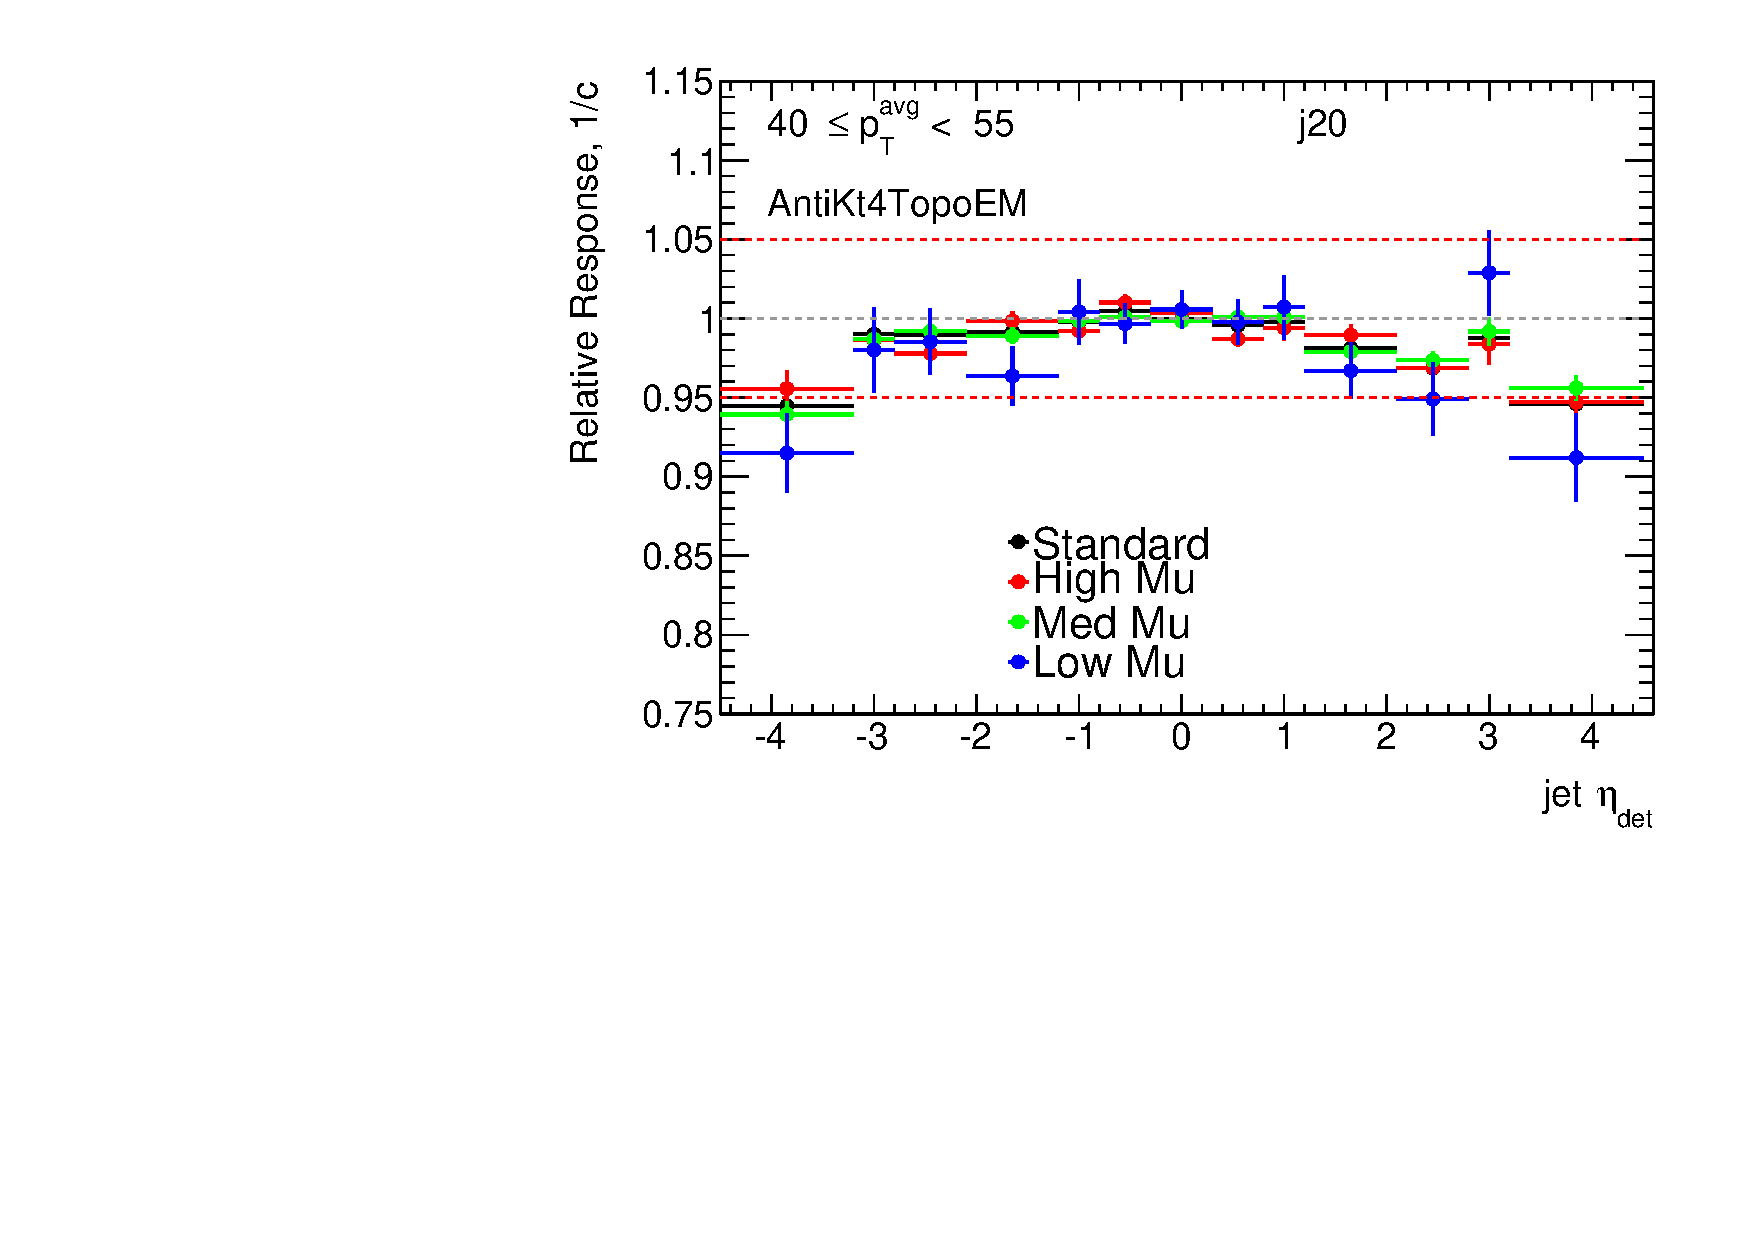
\includegraphics[width=0.8\textwidth]{figures/JetPerformance/2011/Pileup/MuComp_AntiKt4TopoEM_j20_40-55Uncorrected.pdf}
}
\caption[Relative response as a function of $\eta$ for 2 different pileup conditions, based on $\mu{}$, for jets with $55<\ptave{}<75$ GeV]{
Relative response as a function of detector $\eta$ for jets with $55<\ptave{}<75$ GeV.
Relative responses are shown for events with \Range{\mu}{0}{6}, $\rm \mu\ge6$ and all $\mu$. 
\label{JetPerf:MuComp_j20}}
\end{figure}

